\documentclass{article}
\author{Alejandro Zubiri}
\date{Wed Oct 16 2024}
\title{Tema2}

\usepackage{amsmath, amsthm, amsfonts, graphicx}
\graphicspath{{../images/}}

\begin{document}
\maketitle
\tableofcontents
\pagebreak
Este tema desarrollará dos variables simultáneas.\\
\begin{equation}
    \begin{split}
        x=\{ x_{1},\dots,x_{n} \}\\
        y=\{ y_{1},\dots, y_{n} \}
    \end{split}
\end{equation}
\section{Definiciones}
\begin{itemize}
    \item Frecuencia absoluta del par: $f_{ij}$
    \item Frecuencia relativa del par: $fr_{ij}= \frac{f_{ij}}{n}$
    \item Distribución conjunta: valores y frecuencias de los pares.
    \item Distribución marginal: distribución de las variables por separado:
    \begin{equation}
        \begin{split}
            f(x_{i})= \sum ^s f_{ij}\\
            f(y_{j})= \sum ^r f_{ij}
        \end{split}
    \end{equation}
\end{itemize}
\subsection{Distribución condicionada}
Condicionada a que $x$ o $y$ tome un determinado valor:
\begin{equation}
    \begin{split}
        fr(y_{j}| x=x_{i})= \frac{f(x_{i}, y_{j})}{f(x_{i})}
    \end{split}
\end{equation}
\subsection{Variables independientes}
El conocimiento de una no afecta a la otra. Se cumple si
\begin{equation}
    \begin{split}
        fr(y_{j}|x=x_{i})=fr(y_{j})
    \end{split}
\end{equation}
Además, se cumplirá que
\begin{equation}
    \begin{split}
        fr(x_{i},y_{j})=fr(x_{i})\cdot fr(y_{j})
    \end{split}
\end{equation}
Esto es la \textbf{condición de independencia}.
\section{Representación gráfica}
Utilizaremos el diagrama de dispersión:
\begin{center}
    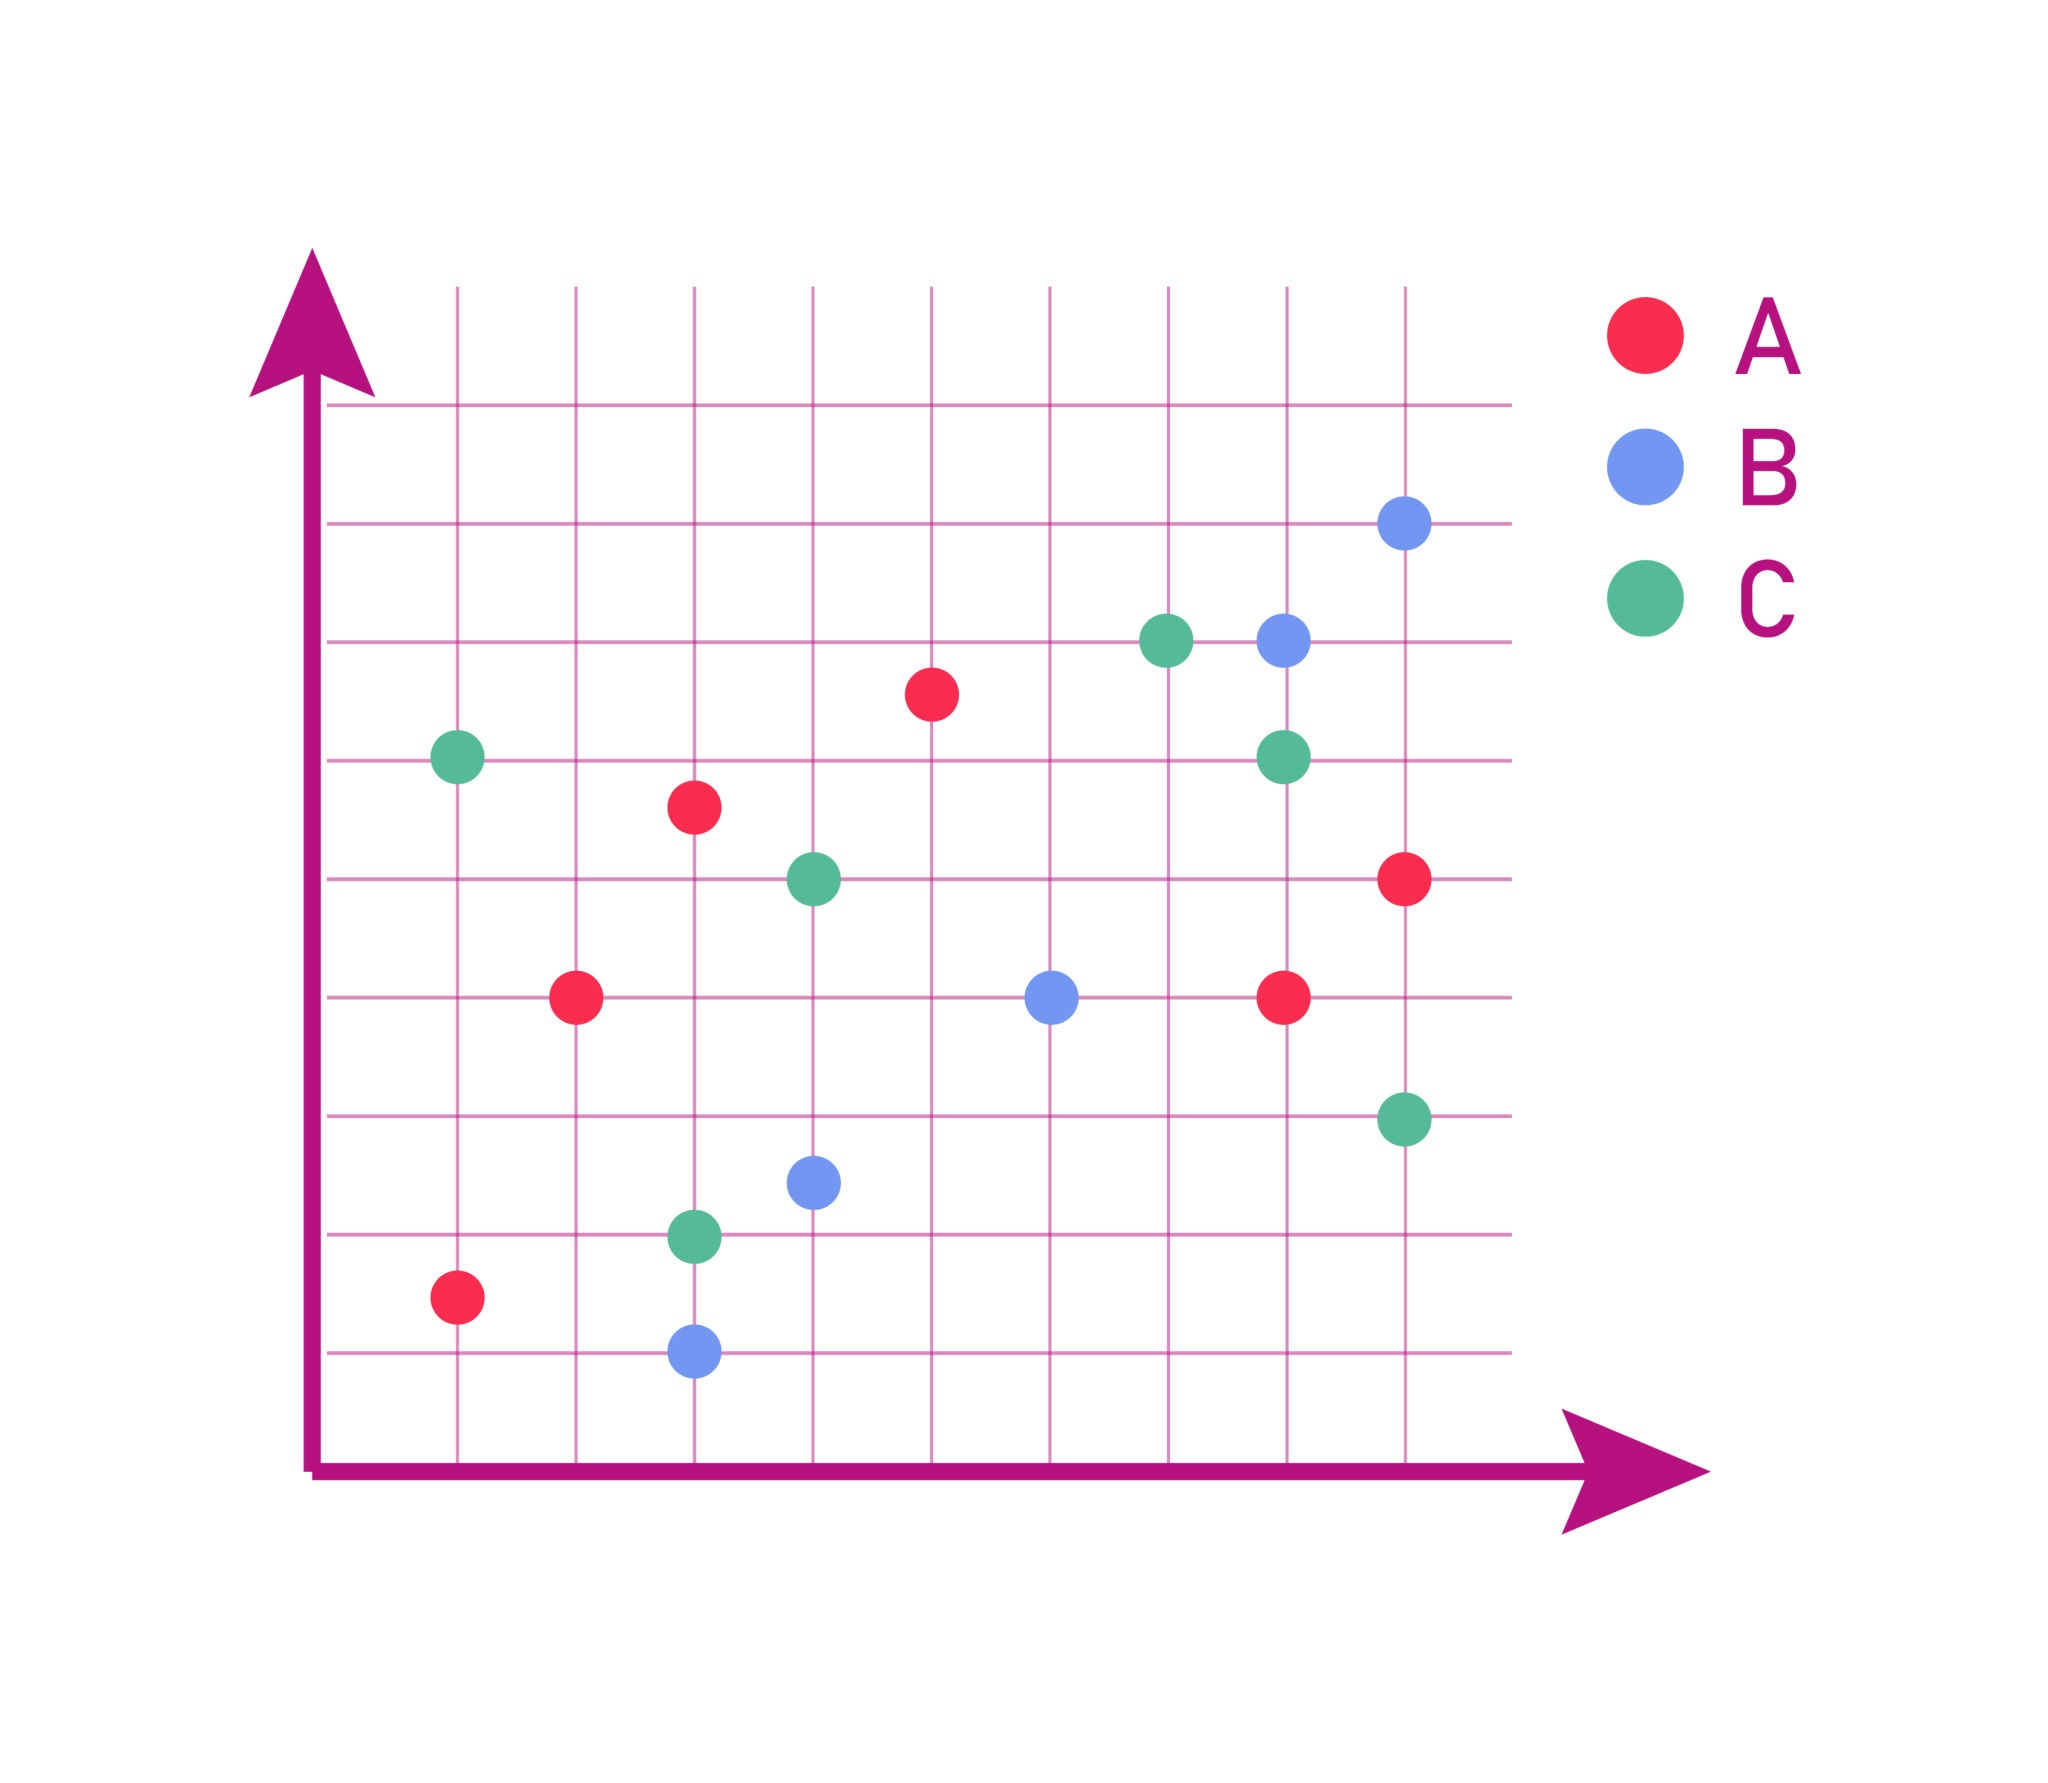
\includegraphics[scale=0.1]{dispersion}
\end{center}
\section{Tipos de covariación}
\subsection{Relaciones de dependencia}
\begin{itemize}
    \item Causal o unilateral: $x$ afecta a $y$, pero no viceversa.
    \item Interdependencia: $x$ afecta a $y$ y viceversa.
    \item Dependencia indirecta: covariación en función de otras variables.
    \item Concordancia: tener la misma calificación bajo un mismo hecho.
    \item Covariación casual.
\end{itemize}
\subsection{Covarianza}
Relación lineal entre variables.
\begin{equation}
    \begin{split}
        cov(x,y)=s_{xy}= \frac{\sum (x_{i}-\bar{x})(y_{i}-\bar{y})f(x_{i},y_{i})}{n}
        = \frac{\sum x_{i}y_{i}f(x_{i}y_{i})}{n} - \bar{x} \bar{y}
    \end{split}
\end{equation}
Si es
\begin{itemize}
    \item Positiva: pendiente positiva.
    \item Negativa: pendiente negativa.
    \item Cero o casi: no hay relación o no es lineal.
\end{itemize}
\subsection{Coeficiente de correlación}
\begin{equation}
    \begin{split}
        r = \frac{S_{xy}}{S_{x}S_{y}} \implies -1 \leq r \leq 1
    \end{split}
\end{equation}
\section{Medidas características}
\subsection{Vector de medias}
Para variables $k$-dimensionales.
Con $k$ observaciones de un individuo $\mathbf{x}$. Sus componentes son las medias:
\begin{equation}
    \begin{split}
        \mathbf{x}= \begin{bmatrix}
        \bar{x}\\
        \bar{y}\\
        .\\
        \end{bmatrix}= \frac{1}{n} \sum \vec{x}_{i}
    \end{split}
\end{equation}
\subsection{Matriz de varianzas}
\begin{equation}
    \begin{split}
        M= \frac{1}{n} \sum \begin{pmatrix}
        x_{i}-\bar{x}\\
        y_{i}-\bar{y}\\
        z_{i}-\bar{z}
        \end{pmatrix} \begin{pmatrix}
        x_{i}-\bar{x} && y_{i}-\bar{y} && z_{i}-\bar{z}
        \end{pmatrix}
    \end{split}
\end{equation}
\subsection{Varianza efectiva}
La raíz de orden $k$ del determinante de la matriz de varianzas
\begin{equation}
    \begin{split}
        VE = \sqrt[k]{|M|}
    \end{split}
\end{equation}
Definimos la desviación típica afectiva como
\begin{equation}
    \begin{split}
        DM= \sqrt{VE} = |M|^{\frac{1}{2k}}
    \end{split}
\end{equation}
\section{Relación entre variables cualitativas}
\subsection{Q de Yule}
Oscila entre $-1$ y $1$. Se puede utilizar cuando tenemos dos categorías:
\begin{equation}
    \begin{split}
        Q = \frac{f_{11}f_{22}- f_{12}f_{21}}{f_{11}f_{22}+ f_{12}f_{21}}
    \end{split}
\end{equation}
$1$ es asociación perfecta, $0$ no hay, y $-1$ perfecta negativa.
\subsection{Coeficiente de contingencia de la $\chi^{2}$}
Comparamos las frecuencias observadas $f_{ij}$ con las esperadas como
si fueran independientes:
\begin{equation}
    \begin{split}
        e_{ij} = \frac{f_{i\cdot } f_{\cdot j}}{n}
    \end{split}
\end{equation}
Entonces
\begin{equation}
    \begin{split}
        \chi^{2}= \sum _{i=1}^r \sum _{j=1}^{s} \frac{(f_{ij}-e_{ij})^{2}}{e_{ij}}
    \end{split}
\end{equation}
Si son independientes, $\chi^{2}=0$.\\
Si $r=s$:
\begin{equation}
    \begin{split}
        max \chi^{2}=n(s-1)
    \end{split}
\end{equation}
\subsection{Coeficiente de contingencia de Pearson}
\begin{equation}
    \begin{split}
        C = \sqrt{\frac{\chi^{2}}{\chi^{2}+n}}
    \end{split}
\end{equation}
Que varía entre $[0,1)$ según la dimensión de la tabla. El valor máchimo es:
\begin{equation}
    \begin{split}
        C_{\text{max}}= \sqrt{\frac{k-1}{k}}
    \end{split}
\end{equation}
Siendo $k=min(r,s)$
\subsection{Coeficiente de contingencia corregido de Pawlik}
\begin{equation}
    \begin{split}
        C_{\text{corr}}= K^* = \frac{C}{C_{\text{max}}}
    \end{split}
\end{equation}
\subsection{V de Cramer}
\begin{equation}
    \begin{split}
        V = \sqrt{\frac{\chi^{2}}{n[min(r,s)-1]}}
    \end{split}
\end{equation}
Teniendo una escala indicando:
\begin{itemize}
    \item $V \leq 0.2$: débil
    \item $0.2 \leq V \leq 0.6$: moderada
    \item $0.6 \leq V$: fuerte
\end{itemize}
\subsection{T de Tschuprov}
\begin{equation}
    \begin{split}
        T^2 = \frac{\chi^{2}}{n \sqrt{(r-1)(s-1)}} \in [0,1]
    \end{split}
\end{equation}
\subsection{Coeficiente de correlación por rangos de Spearman}
En escala ordinal, oscila entre $[-1,1]$:
\begin{equation}
    \begin{split}
        r_{s}= 1 - \frac{6 \sum d_{i}^{2}}{n(n^{2}-1)}
    \end{split}
\end{equation}
Donde $d_{i}$ es la diferencia de cada par ordenado.
\subsection{Razón de correlación}
Mide el grado entre cualitatica y cuantitativa:
\begin{equation}
    \begin{split}
        \eta^{2}_{y / x} = \frac{\sum f_{\cdot j} (\bar{y_{x}}- \bar{y})^{2}}{n \sigma^{2}_{y}}
    \end{split}
\end{equation}
donde
\begin{itemize}
    \item $f_{\cdot j}$: número de datos por categoría.
    \item $\bar{y_{x}}$: media de la categoría.
\end{itemize}

\end{document}